%!TEX root = ../Main.tex
The conclusion of the preliminary work revolves around the Transmission Routine. Here all the functions producing on-site hamiltonians, full hamiltonians, hopping matrices, bandstructures, self energy and Green's functions by recursion play their part in getting the transmission through the material. \textit{This part is an attempt to describe the basic theory behind transmission/transport and it is very likely to need rework, additions and editing} The transmission tells us the likelihood whether an electron will be transported trough a "device region" at different energies and thus how the "device region" affects the overall current through larger systems. This means that the system will have to be well defined before one can use the functions developed for calculation of the different parts needed for production of transmission. The "device region" contains at least one central unit cell as well as a "left" and "right" unit cell. The left and right unit cell represents the contact region of the device i.e. the two parts that connects to the "rest" of the system/molecule. It is assumed that the contacts represent a system that is made up of unit cells which can be reduced by recursion, though not necessarily identical on each side (left and right). Knowing which "blocks" the system contains and how to obtain them with the already developed functions, three main ingredients are needed to obtain the transmission through a device. The first one is the Green's function for the device region \(\mathbf{G}_D\) for which one needs the device hamiltonian \(\mathbf{H}_D\) as well as the left and right selfenergies \(\mathbf{\Sigma}_L, \ \mathbf{\Sigma}_R\). The left and right selfenergies constitutes the second ingredient and can be obtained through left and right hopping matrices as well as the left and right on-site Green's functions. The last main ingredient are \(\mathbf{\Gamma}_L,\ \mathbf{\Gamma}_R\) which are matrix operators describing the coupling between the left and right parts of hilbert space. They are called rate equations because..... The rate equation are obtained via the self energies in the following fashion: 
\begin{align}
\mathbf{\Gamma}_{L/R} = i(\mathbf{\Sigma}_{L/R} - \mathbf{\Sigma}^{\dagger}_{L/R})
\end{align}To give an overview of how the different matrices are defined in relation to a system an illustration has been made.See \cref{systemillu}. Using the Green's function, left/right self energies as well as the left/right rate matrices, the transmission, as a function of energy, can be obtained via the following equation:
\begin{align}
    T(E) = \text{Tr}[\mathbf{\Gamma}_R\mathbf{G}_D\mathbf{\Gamma}_L\mathbf{G}_D^{\dagger}](E)
\end{align}
Where Tr is the trace of the matrix product. 
\begin{figure}
    \centering
    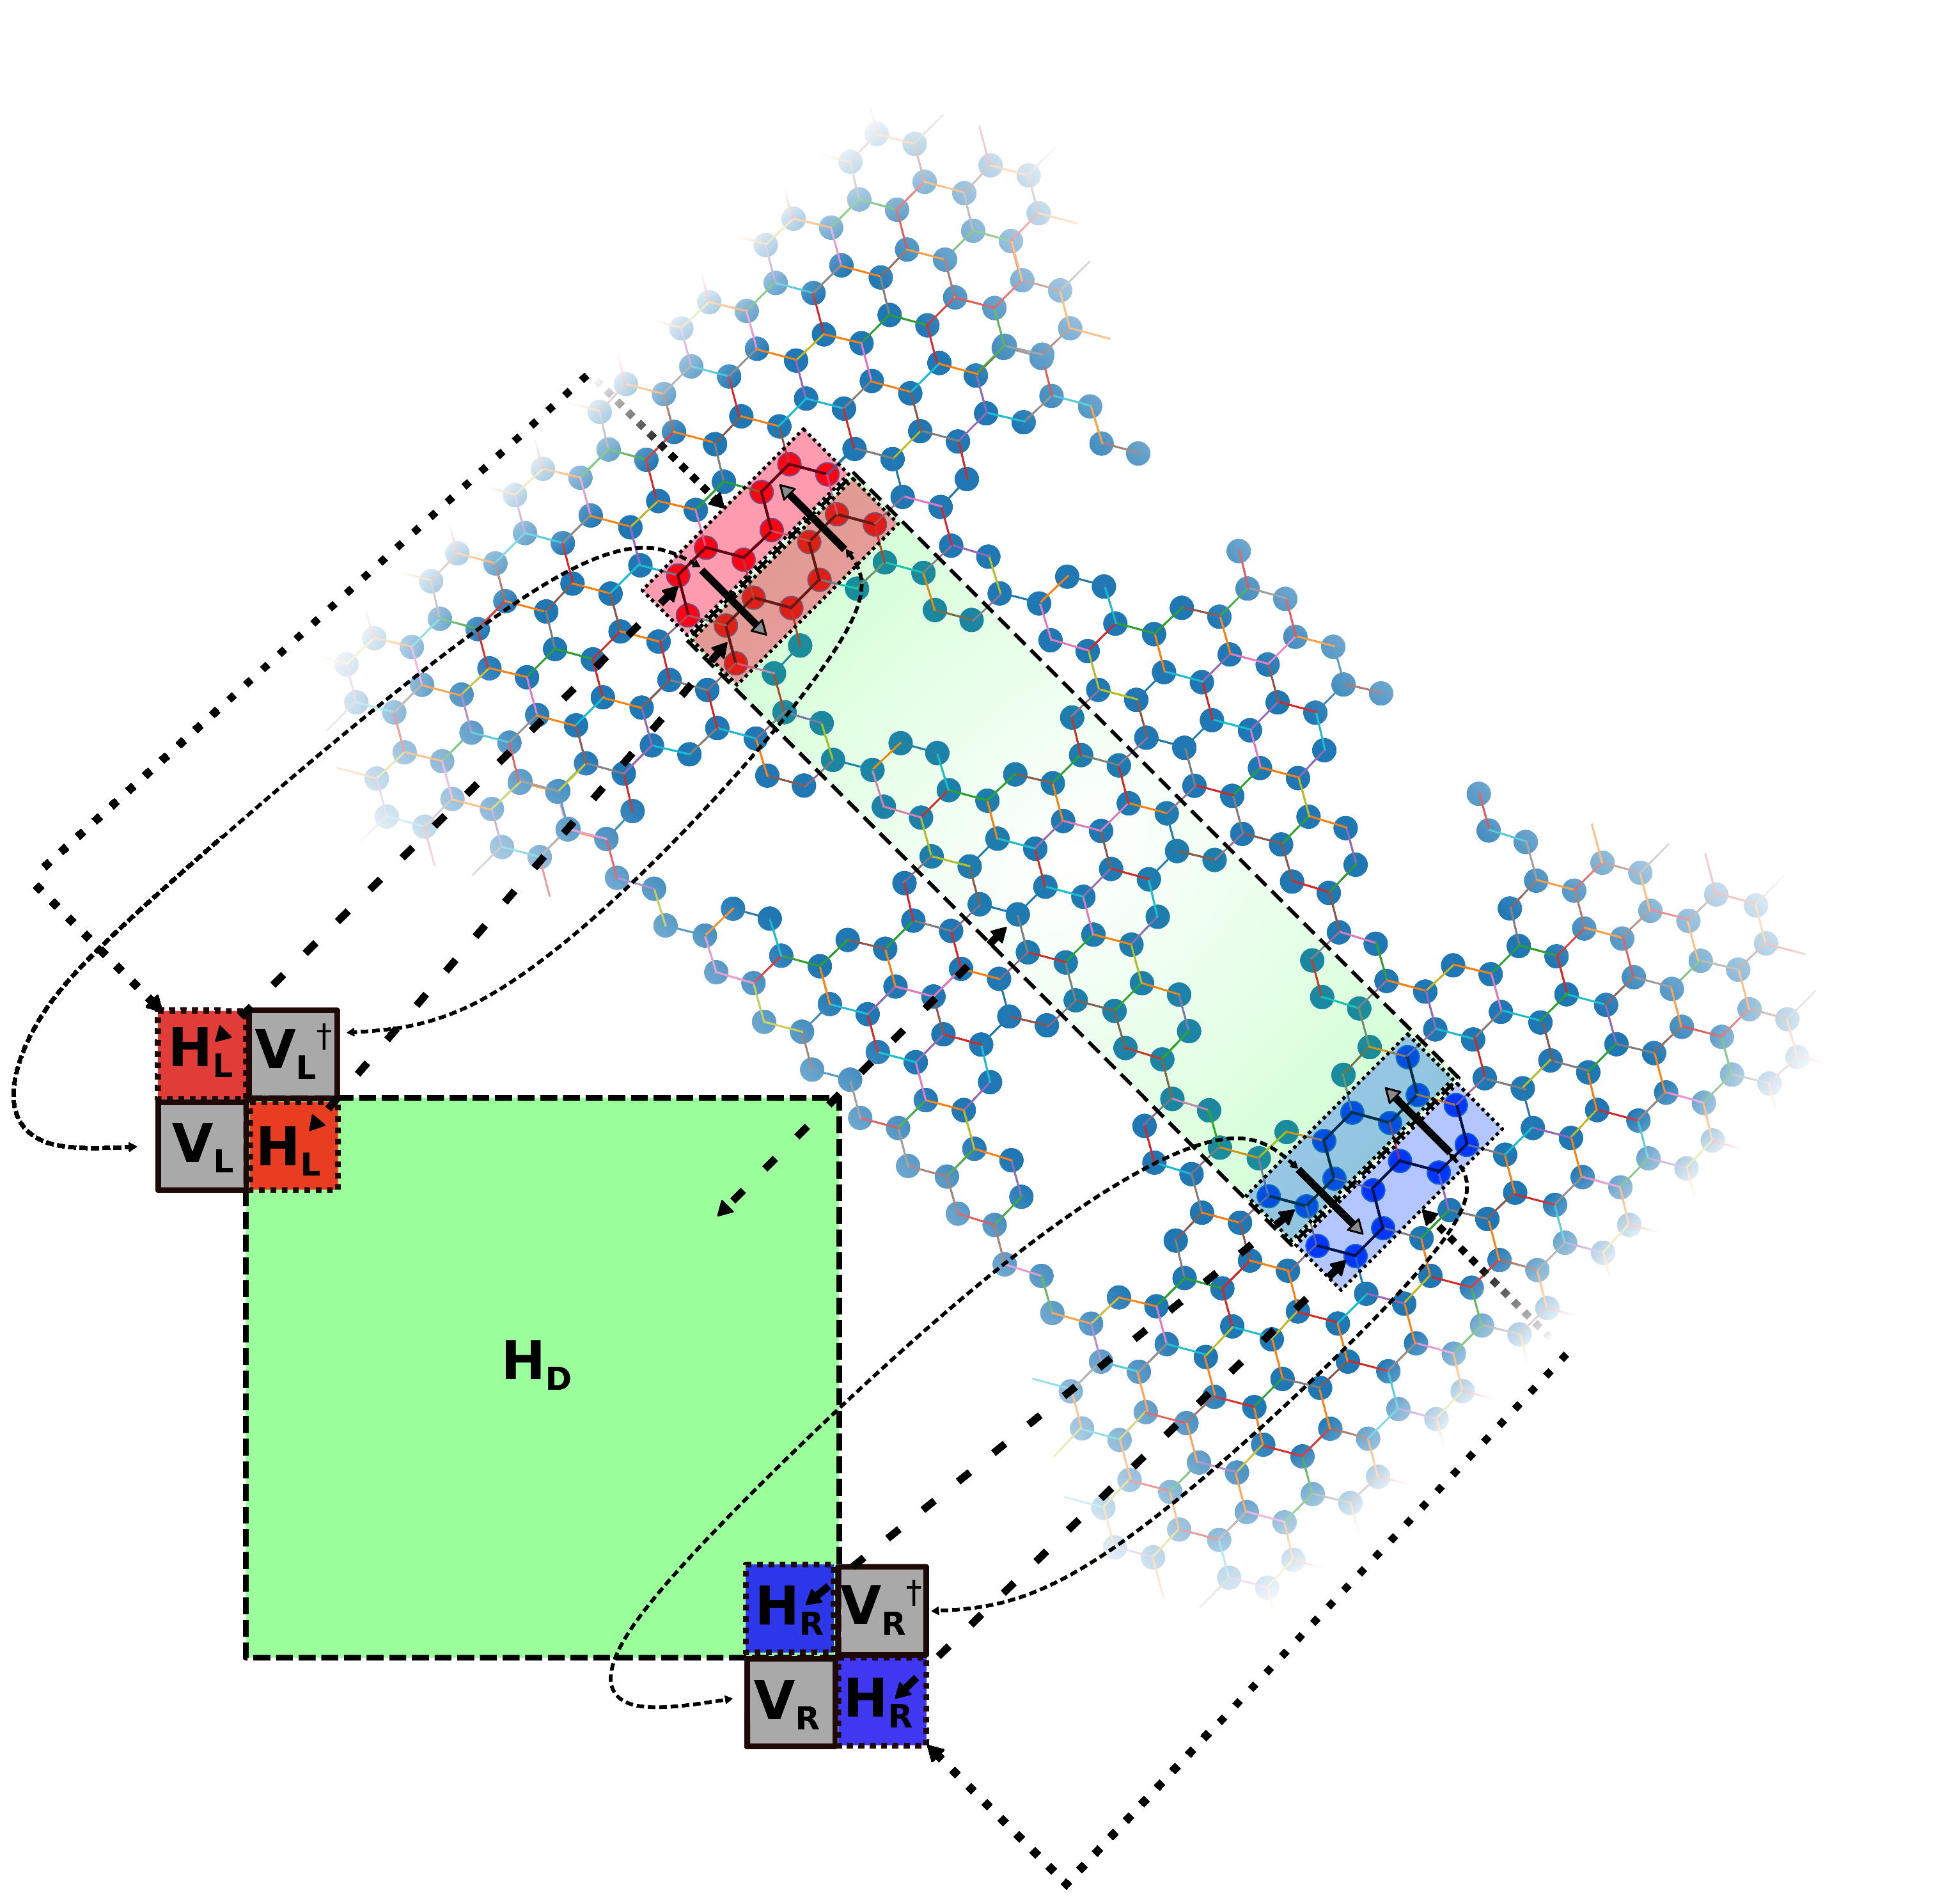
\includegraphics[width=0.9\textwidth]{Listings/illu.eps}
    \caption{Illustration showing how the different parts of the system are translated into matrix blocks. On the graphene the green box is the unit cell of the device. It includes one red and blue box which themselves are unit cells of the left and right contacts. These unit cells can be translated into hamiltonian matrices \(\textbf{H}_D, \ \textbf{H}_L,\ \textbf{H}_R\) as illustrated. Note that because the first of the left and right unit cells (red and blue) are inside the device (green region), they can be picked out of \(\textbf{H}_D\) directly and so it is not necessary to make them from scratch. The two other unit cells lying outside the device region represents what could be an infinite contact region. The contact region is therefore potentially of an infinitely bigger dimension compared to the device region, however, by recursion, this region can be collapsed into a single hamiltonian of same dimension as the one inside the device region. Finally the two fat black arrows on each side of the device represents the hopping between the device and contact region. Note that the direction of hopping corresponds to a specific hopping matrix. F.ex. left-to-right is the ordinary hopping matrix while right-to-left is its conjugate (for both left and right).}
    \label{systemillu}
\end{figure}
\subsection{Transmission in 1D a simple example}
As with the Recursion Routine, the development of this routine will be build up around a small system in order to make sure that the obtained results are as expected, thereafter generalising the routine to suit all kinds and sizes of system.

